% !TEX program = xelatex

\documentclass[10pt,aspectratio=169]{beamer}
\usetheme[
    hidetitle,           % hide the (short) title in the sidebar
    hideauthor,          % hide the (short) author in the sidebar
    hideinstitute,       % hide the (short) institute in the bottom of the sidebar
    left                 % right of left position of sidebar
  ]{Aalborg}

%\setbeamercolor{alerted text}{fg=beamer@headercolor}

\usepackage[british]{babel}
\usepackage[babel,english=british]{csquotes}
\usepackage{datetime}
\usepackage[version=4]{mhchem}
\usepackage{booktabs}
\usepackage{xspace}
\usepackage{multicol}
\usepackage{graphicx}
\usepackage{tikz}
\usepackage{hyperref}
\newcommand{\doi}[1]{\href{https://doi.org/#1}{doi:#1}}


%\setbeamercolor{section in sidebar current subsection}{use=section in sidebar,fg=section in sidebar.fg,bg=section in sidebar.bg}
% Direct graphics path to the figures folder of the dissertation
\graphicspath{{../figures/}}

\usepackage{fontspec}
\usepackage{lmodern}
\IfFileExists{../font/LinotypeSyntaxCom-Regular.ttf}{
  \setsansfont{LinotypeSyntaxCom}[
    Path=../font/,
    Extension = .ttf,
    UprightFont=*-Regular,
    BoldFont=*-Bold,
    ItalicFont=*-Italic,
    BoldItalicFont=*-BoldIt
  ]
}{
  \usepackage{lmodern}
}

\usepackage{animate}
\usepackage[version=4]{mhchem}
\usepackage{orcidlink}

% Dummy command for potential background images from the template
%\newcommand{\BUWtitlebg}{}

\title[Dissertation]
{Advanced 2D and 3D characterisation of clinker phases and hydrated cementitious binders}

\subtitle{Overview of the Thesis}

% Anwendung des Formats
\date{10$^\text{th}$ June 2026}

\newcommand\shortauthor{Florian Kleiner}
\newcommand\orcid{0000-0001-6002-0829}
\author[\shortauthor]{
  \shortauthor\,\orcidlink{\orcid}\\
  \href{mailto:florian.kleiner@uni-weimar.de}{{\tt florian.kleiner@uni-weimar.de}}
}

\institute[Bauhaus-Universität Weimar]{
  Bauhaus-Universität Weimar\\
  Fak. B\&U\\
  Prof. Werkstoffe des Bauens
}

\begin{document}

% ---------------------------------------------------
% Slide 1: Title Slide
% ---------------------------------------------------
{\BUWtitlebg
\begin{frame}[plain,noframenumbering]
  \titlepage

\end{frame}}


\section{Motivation}
\begin{frame}{Motivation \& Objectives}
  \begin{itemize}
    \item Cement hydration is a highly complex process.
    \item Classical individual methods reach their limits regarding the resolution of nano-pore spaces, chemical trace elements, or phase assignment.
  \end{itemize}
  
  \begin{center}
    \animategraphics[palindrome,autoplay,width=.75\textwidth]{6}{intro-anim/Animation}{01}{10}
  \end{center}
\end{frame}


\section{Methods}
\begin{frame}{Methods}
  \textbf{The goal is to overcome these limits through:}
  \begin{itemize}
    \item Application of correlative microscopy.
    \item Automation of evaluation and image analysis.
    \item Comparison of different methods.
  \end{itemize}
  \begin{center}
    \begin{tabular}{lll}
      \toprule
      \textbf{Preparation} & \textbf{Imaging} & \textbf{Physical} \\
      \midrule
      ArBIB & SEM-BSE/SE & Nanoindentation (NI) \\
      Cryo-FIB & EDX \& EBSD & LT-DSC \\
      fs-Laser & LA-ICP-MS & MIP \\
       & FIB-nT & \\
      \bottomrule
    \end{tabular}
  \end{center}
  
  \begin{itemize}
    \item Focus on preserving the native microstructure.
  \end{itemize}
\end{frame}


\section{ArBIB Preparation}
\begin{frame}{Argon Broad Ion Beam (ArBIB) milling}
  \begin{columns}
    \begin{column}{0.5\textwidth}
      \begin{itemize}
        \item Large-area polishing of hydrated specimens without embedding.
        \item Improved pore segmentability with resin embedding.
        \item Enables visualisation of nano-pores within the dense C-S-H structure.
        \item Cryo-ArBIB reduces thermal damage to hydrate phases.
      \end{itemize}
    \end{column}
    \begin{column}{0.5\textwidth}
      \centering
      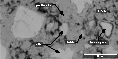
\includegraphics[width=\linewidth]{literature/ArBIB-CEMI-BSE.pdf}\\
      \footnotesize ArBIB-milled, 28\,d hydrated CEM I\\

    \end{column}
  \end{columns}
  \vfill\raggedleft\tiny\itshape F. Kleiner, C. Matthes, C. Rößler, `Argon broad ion beam sectioning and high resolution scanning electron microscopy imaging of hydrated alite', 2021, \doi{10.1016/j.cemconres.2021.106583}
\end{frame}


\section{Correlative Microscopy}
\subsection{BSE + EDX + LA-ICP-MS}
\begin{frame}{Trace Element Analysis in Clinker}
  \begin{columns}
    \begin{column}{0.5\textwidth}
      \textbf{BSE + EDX + LA-ICP-MS}
      \begin{itemize}
        \item High resolution of EDX data enables precise phase assignment of LA-ICP-MS measurements.
        \item Trace elements such as V, Ba, Rb are concentrated in \ce{C2S}, while Ti and Mn are found in the interstitial phases.
      \end{itemize}
    \end{column}
    \begin{column}{0.5\textwidth}
      \centering
      \animategraphics[loop,autoplay,width=\linewidth]{1}{la-icp-ms/position2-anim/Animation}{0}{4}\\
      \footnotesize Position of EDX and LA-ICP-MS measurements.\\

    \end{column}
  \end{columns}
   \vfill\raggedleft\tiny\itshape F. Kleiner, M. Decker, C. Rößler, H. Hilbig, H.-M. Ludwig, `Combined LA-ICP-MS and SEM-EDX analyses for spatially resolved major, minor and trace element detection in cement clinker phases', 2022, \doi{10.1016/j.cemconres.2022.106875}
\end{frame}

\subsection{Nanoindentation + EDX}
\begin{frame}{Nanoindentation (NI) + EDX}
  \begin{columns}
    \begin{column}{0.5\textwidth}
      \textbf{Mechanical Properties of Mortars}
      \begin{itemize}
        \item Preparation via ArBIB.
        \item Reduced preparation artefacts (avoidance of relief).
        \item Combination of NI + EDX.
        \item Direct, detailed phase assignment of hardness/modulus (e.g. quartz, \ce{C3S}, \ce{C2S}, C-S-H, C-A-S-H) in contrast to the commonly used coarse deconvolution methods.
      \end{itemize}
    \end{column}
    \begin{column}{0.5\textwidth}
      \centering
      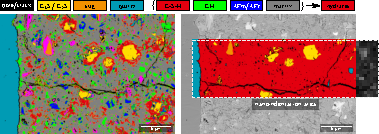
\includegraphics[width=.8\linewidth]{nanoindentation/EDX_positions.pdf}\\
      \footnotesize EDX phase map, registered on a BSE image\\at the location of the NI experiments.\\
      \vspace{0.15cm}
      \animategraphics[loop,autoplay,width=.8\linewidth]{1}{./graphics/NI/0}{0}{2}\\
      \footnotesize EDX phase map, registered on the hardness map ($H$)\\
    \end{column}
  \end{columns}
  \vfill\raggedleft\tiny\itshape unpublished
\end{frame}



\section{Hydrate Layer and Distance Measurements}
\subsection{Hydrate Layer Measurements}
\begin{frame}{Hydrate Layer Thickness (HLT) Measurements}
  \begin{columns}
    \begin{column}{0.5\textwidth}
      \begin{itemize}
        \item Development of an algorithm for HLT measurement on large-scale BSE images.
        \item Via coordinate transformation (Cartesian to polar).
        \item Enables the measurement of hydration progress on hundreds of thousands of particles.
      \end{itemize}
    \end{column}
    \begin{column}{0.5\textwidth}
      \centering
      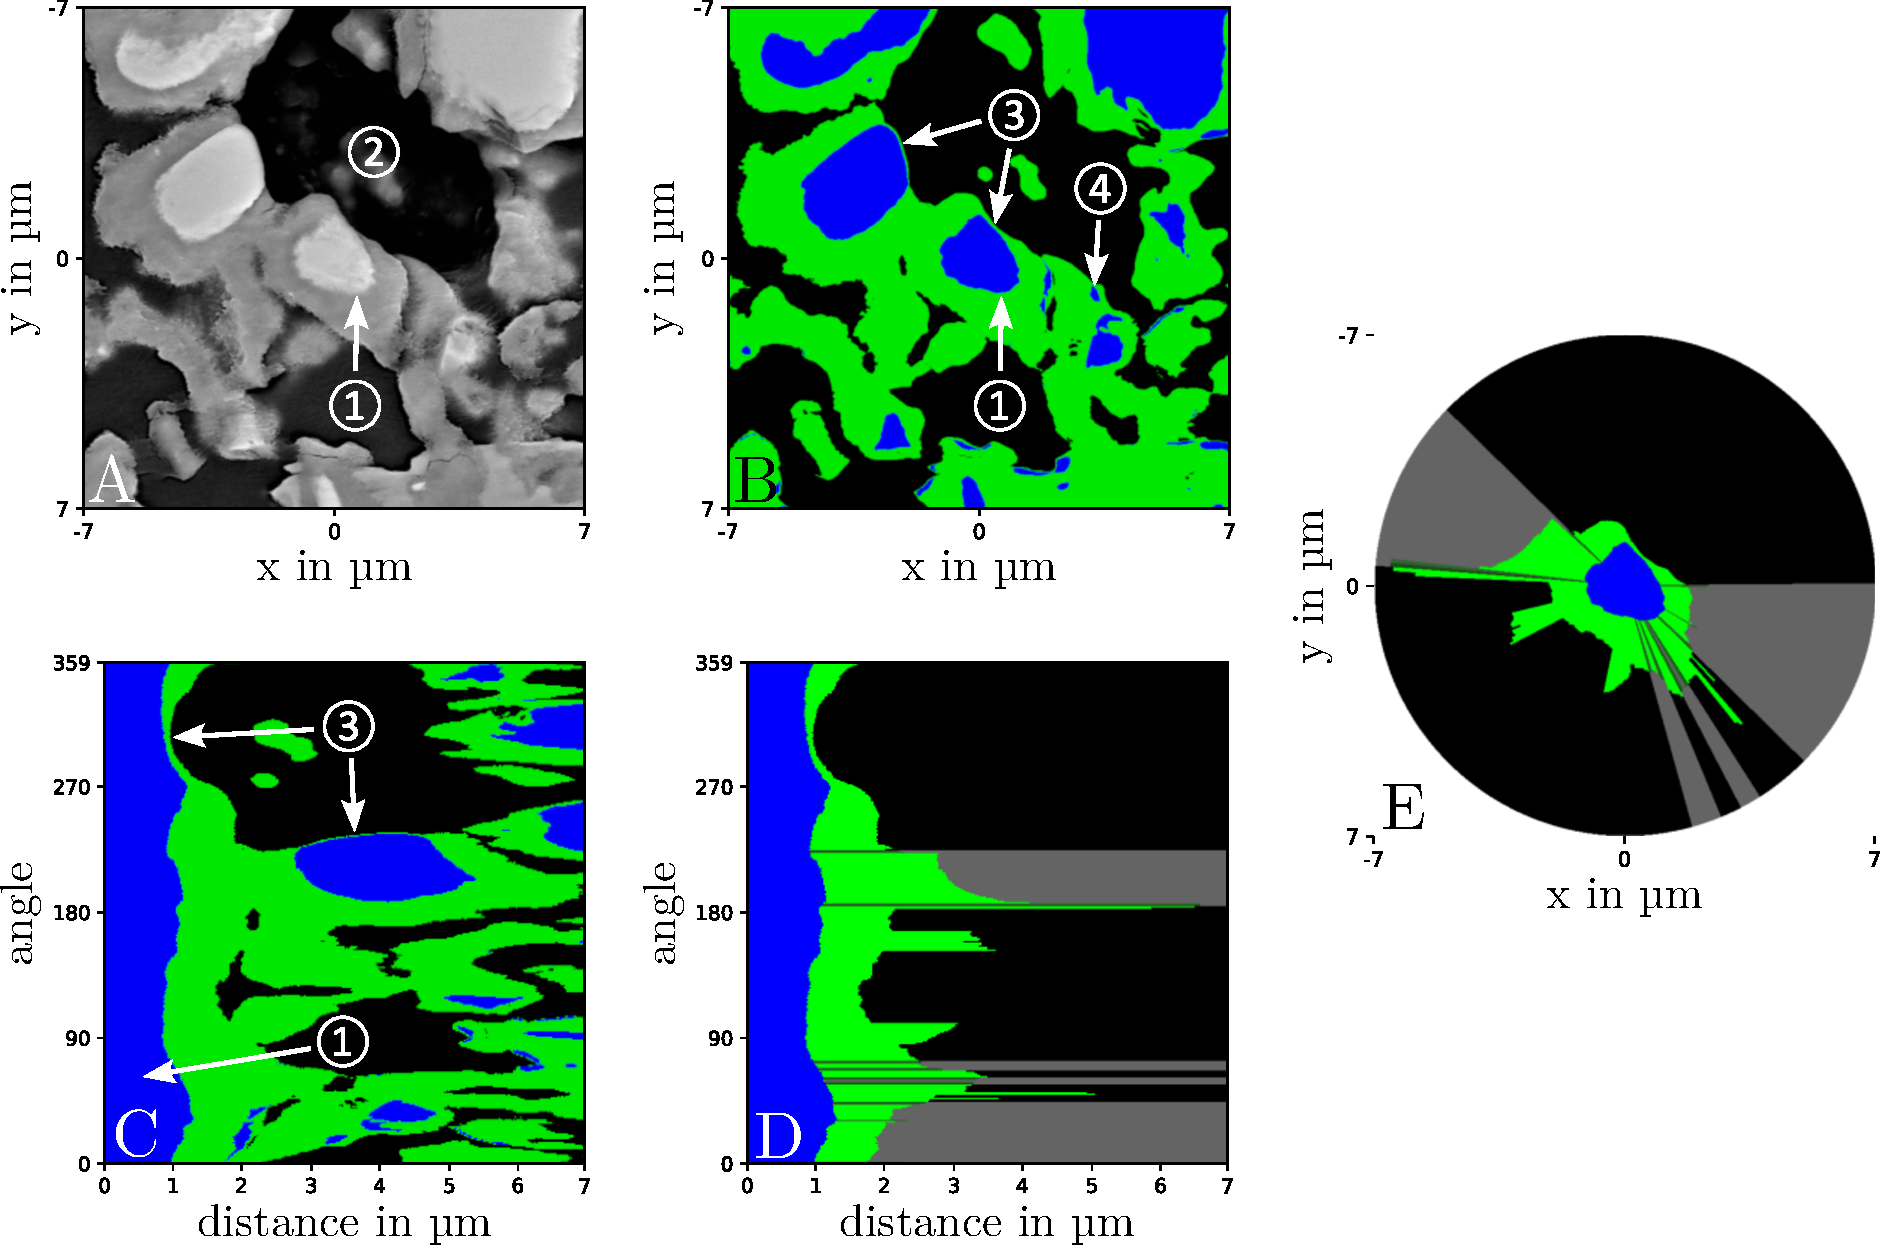
\includegraphics[width=0.9\linewidth]{hydrate-rim/Mechanism_v2.pdf}
      \footnotesize Illustration of the HLT measurement\\using a clinker grain as an example.
    \end{column}
  \end{columns}
   \vfill
   \raggedleft\tiny\itshape F. Kleiner, F. Becker, C. Rößler, H.-M. Ludwig, `A Python tool to determine the thickness of the hydrate layer around clinker grains using SEM-BSE images.', 2024, \doi{10.1111/jmi.13283}
\end{frame}


\begin{frame}{Hydrate Layer Thickness (HLT) Measurements}
  \begin{columns}
    \begin{column}{0.5\textwidth}
      \textbf{Results for \ce{C3S} and \ce{C2S}:}
      \begin{itemize}
        \item For pure phases (\ce{C3S} and \ce{C2S}), HLT growth is measurable in specimens up to 28 days old.
        \item \ce{C2S} shows expectedly slower C-S-H growth than \ce{C3S}.
        \item For mixed phases (\ce{C3S}:\ce{C2S} 3:1, 1:1, 1:3), distinct growth rates around \ce{C3S} and \ce{C2S} can be determined.
      \end{itemize}
    \end{column}
    \begin{column}{0.5\textwidth}
      \centering
      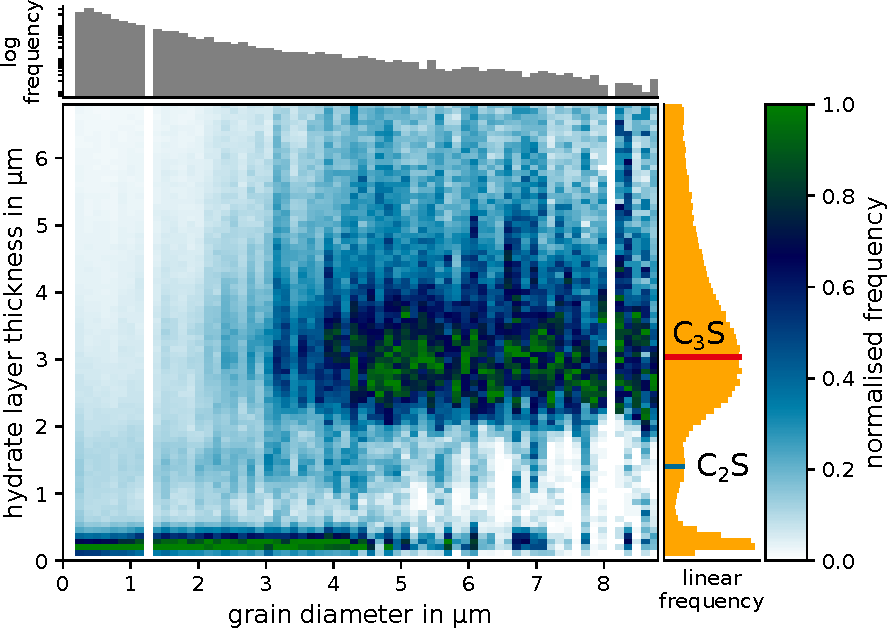
\includegraphics[width=\linewidth]{hydrate-rim/HLT_histogram_3-1.pdf}
      \footnotesize HLT result for 28\,d hydrated \ce{C3S}:\ce{C2S} 3:1. In the HLT histogram (orange), the peaks (green) can be assigned to \ce{C2S} and \ce{C3S}.\\
    \end{column}
  \end{columns}
\end{frame}

\subsection{EBSD \& HLT Correlation}
\begin{frame}{EBSD \& HLT Correlation}
  \begin{columns}
    \begin{column}{0.4\textwidth}
      Does C-S-H grow preferentially on specific \ce{C3S} crystal faces?
      \begin{itemize}
        \item Acquistion of a BSE image for HLT measurement.
        \item Measurement of the crystal orientation of unhydrated \ce{C3S} particles using electron backscatter diffraction (EBSD).
      \end{itemize}
    \end{column}
    \begin{column}{0.6\textwidth}
      \centering
      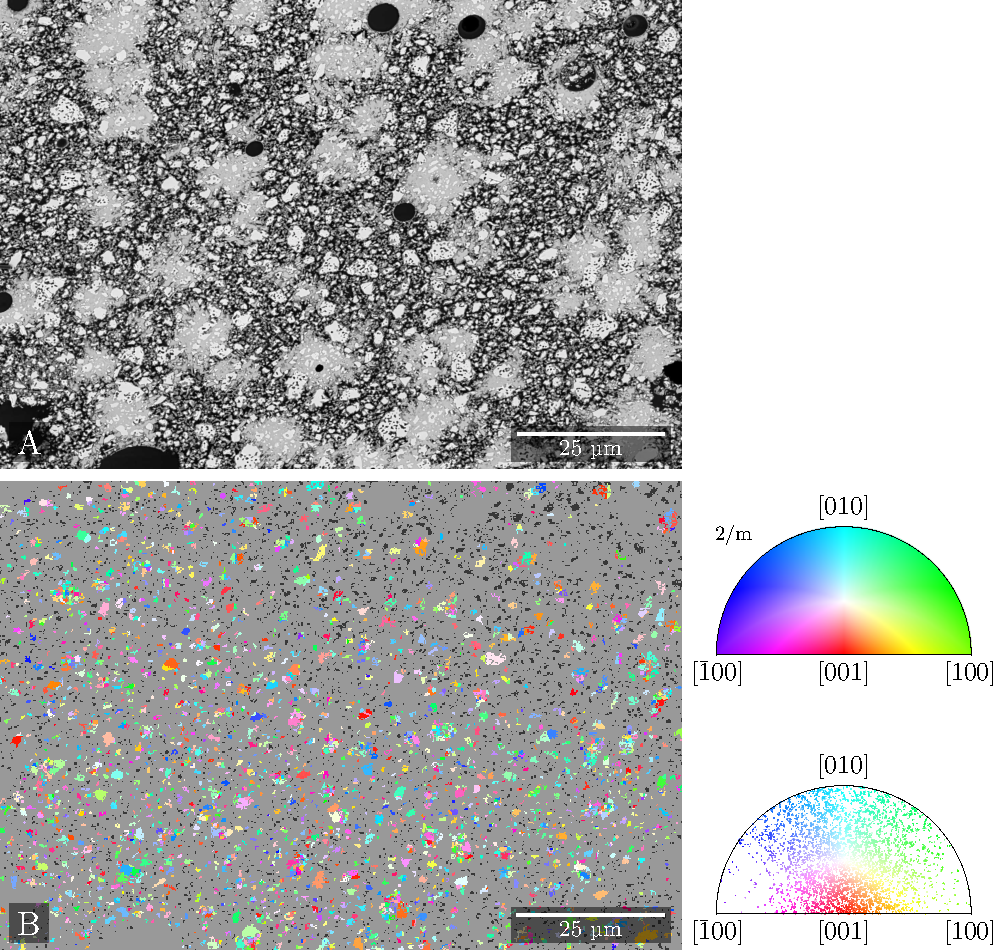
\includegraphics[width=.65\textheight]{./graphics/ebsd/BSE+EBSD-site5.pdf}\\
      \footnotesize BSE (top) and EBSD mapping (bottom)\\with IPF-Z key and IPF-Z distribution
    \end{column}
  \end{columns}
  \vfill\raggedleft\tiny\itshape unpublished
\end{frame}

\begin{frame}{EBSD \& HLT Correlation}
  \begin{columns}
    \begin{column}{0.4\textwidth}
      \textbf{Results:}
      \begin{itemize}
        \item No significant crystallographic preference found.
        \item Significant dependence of measurement density on the crystallographic orientation.
        \item The local environment (pore space) dominates the growth.
      \end{itemize}
    \end{column}
    \begin{column}{0.6\textwidth}
      \centering
      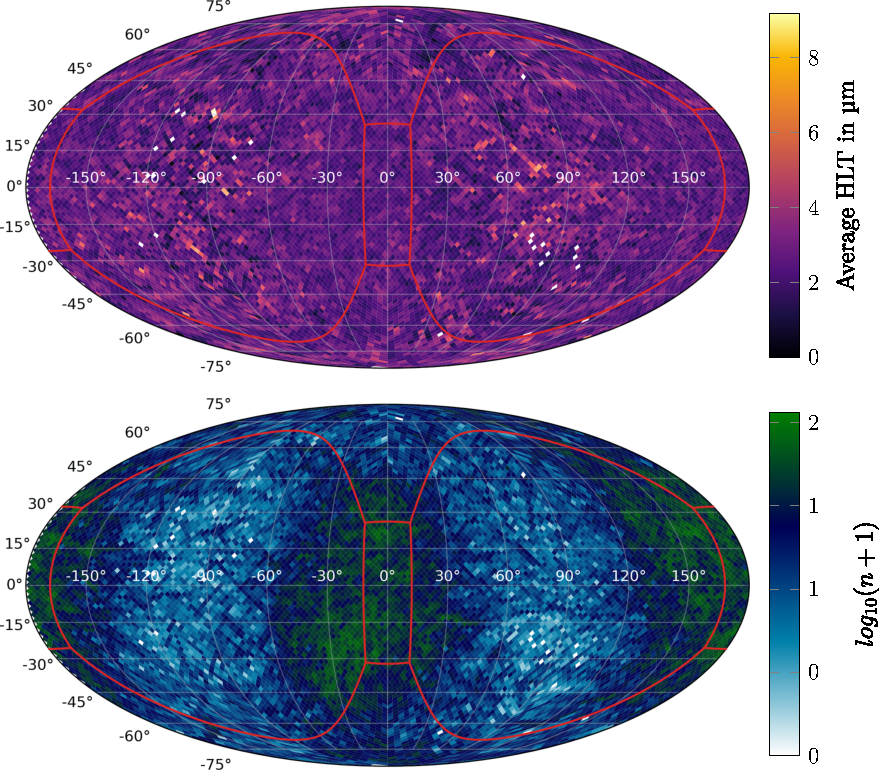
\includegraphics[width=0.7\linewidth]{./graphics/ebsd/mollweideprojektion.pdf}\\
      \footnotesize Mollweide projection of the mean HLT (top) and the measurement density (bottom) with projected \ce{C3S} unit cell (MIII polymorph, red).
    \end{column}
  \end{columns}
  \vfill\raggedleft\tiny\itshape unpublished
\end{frame}

\subsection{Particle Distance Measurement}
\begin{frame}{Particle Distances (Fresh Paste)}
  \begin{columns}
    \begin{column}{0.5\textwidth}
      \begin{itemize}
        \item Preparation via cryo-FIB-SEM to preserve the native microstructure.
        \item Adaptation of the HLT algorithm to determine particle distances.
      \end{itemize}
      \vspace{0.5cm}
      \textbf{Results:}
      \begin{itemize}
        \item Objective quantification of the dispersing effect.
        \item Effects of power ultrasound (PUS) and superplasticisers (PCE) are measurable.
      \end{itemize}
    \end{column}
    \begin{column}{0.5\textwidth}
      \centering
      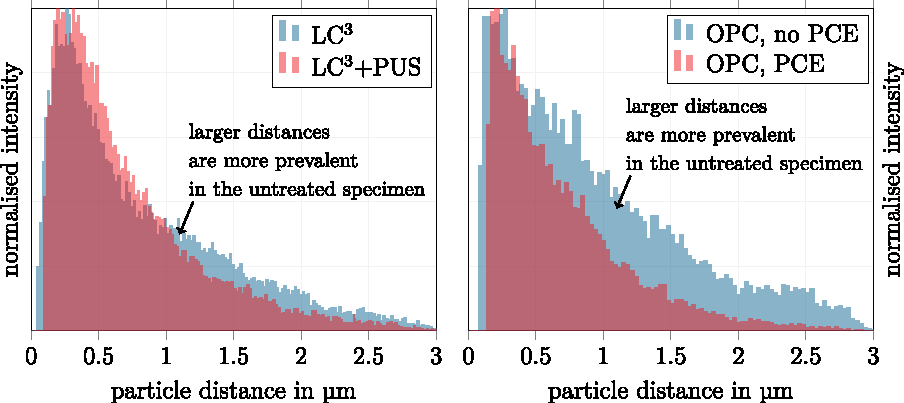
\includegraphics[width=\linewidth]{./graphics/particledistance/diagram.pdf}
      \footnotesize Particle distance distribution of LC$^3$ (left)\\and Portland cement pastes (right)\\with and without the use of PUS or PCE.
    \end{column}
  \end{columns}
  \vfill\raggedleft\tiny\itshape unpublished
\end{frame}

    
\section{3D FIB-SEM}    
\subsection{Lift-out Technique}
\begin{frame}{3D Nano Tomography (FIB-nT) - Lift-out}
  \begin{columns}
    \begin{column}{0.5\textwidth}
      \textbf{Challenges:}
      \begin{itemize}
        \item Artefacts in the bulk material (charging, curtaining).
      \end{itemize}
      \textbf{The Solution:}
      \begin{itemize}
        \item Lift-out technique.
        \item Segmentation using 3D SLIC superpixels \& UMAP clustering.
        \item MIP/LT-DSC validation in the range of $\approx$\,10\,nm.
      \end{itemize}
    \end{column}
    \begin{column}{0.5\textwidth}
      \centering
      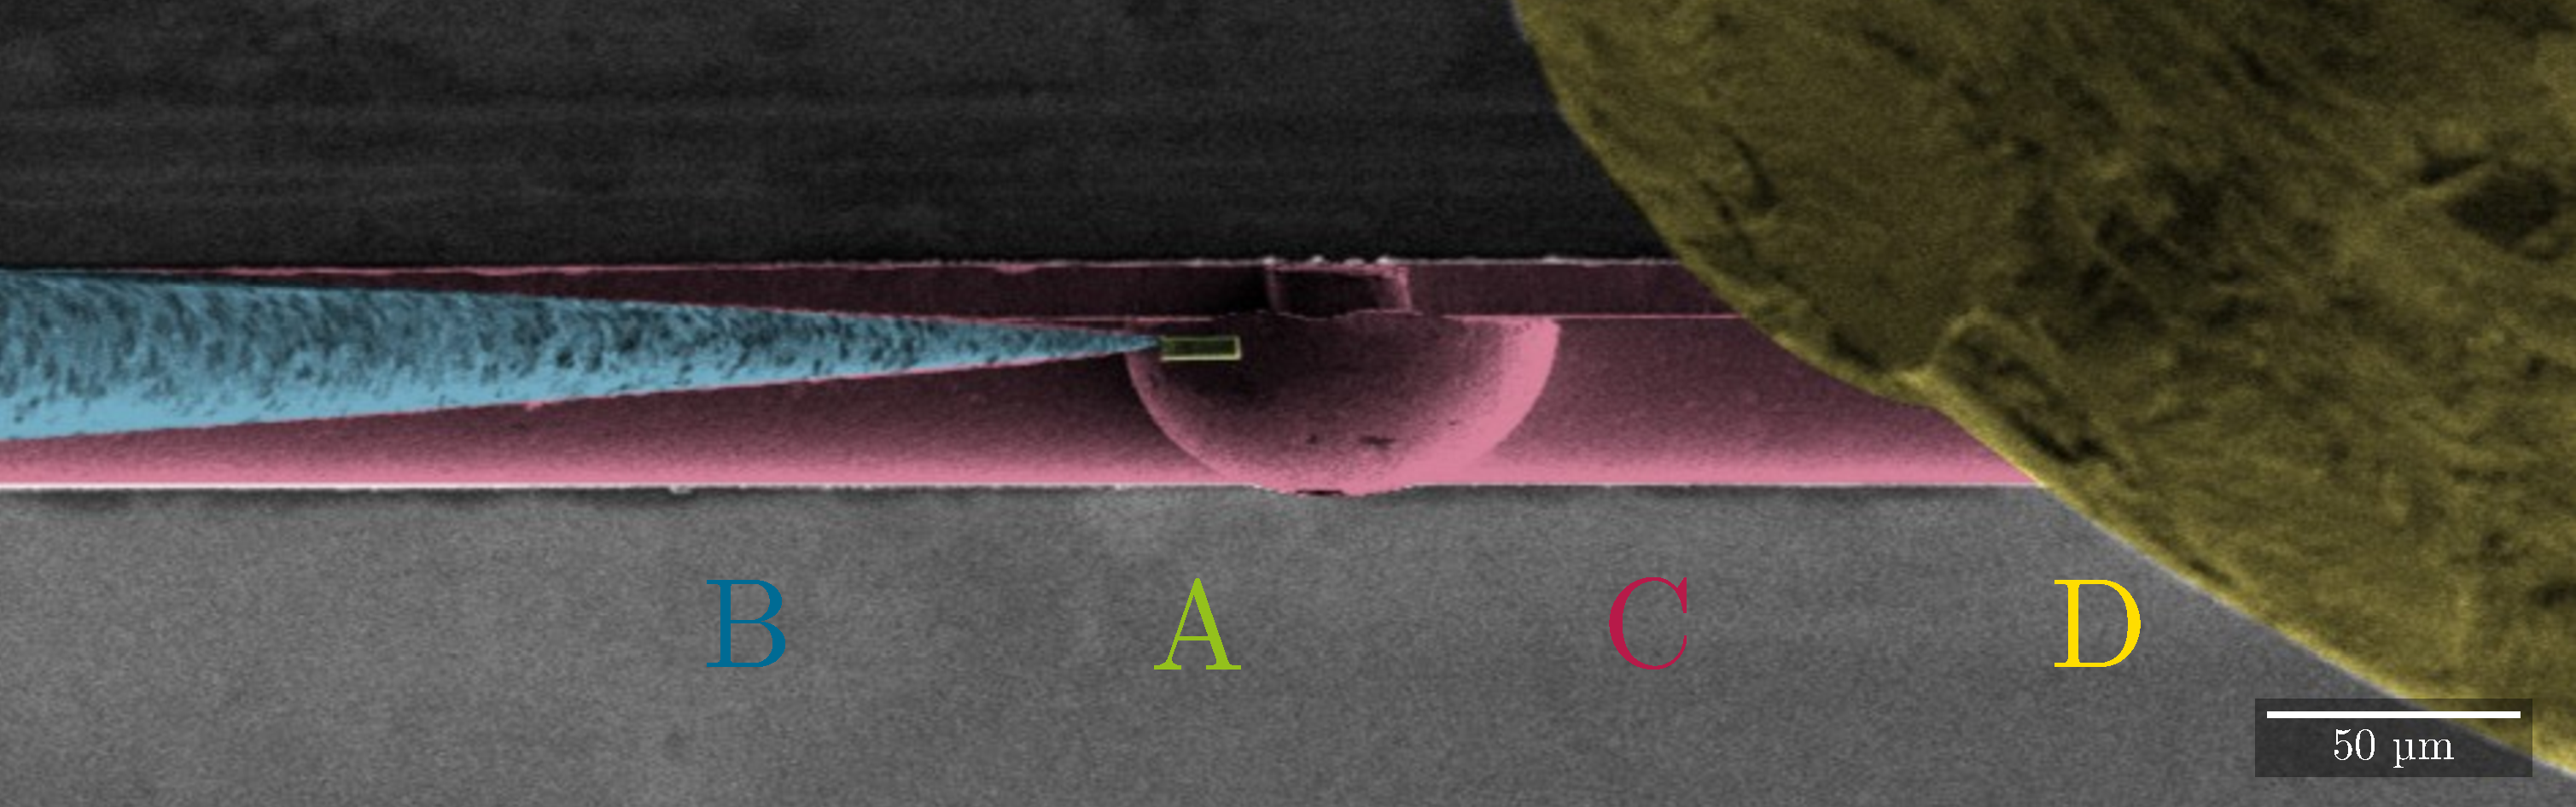
\includegraphics[width=0.9\linewidth]{methods/fib_liftout/image095_colored.pdf}
      \footnotesize Lift-out principle. A sample, B needle, C copper comb, D platinum deposition system\\[0.2cm]
      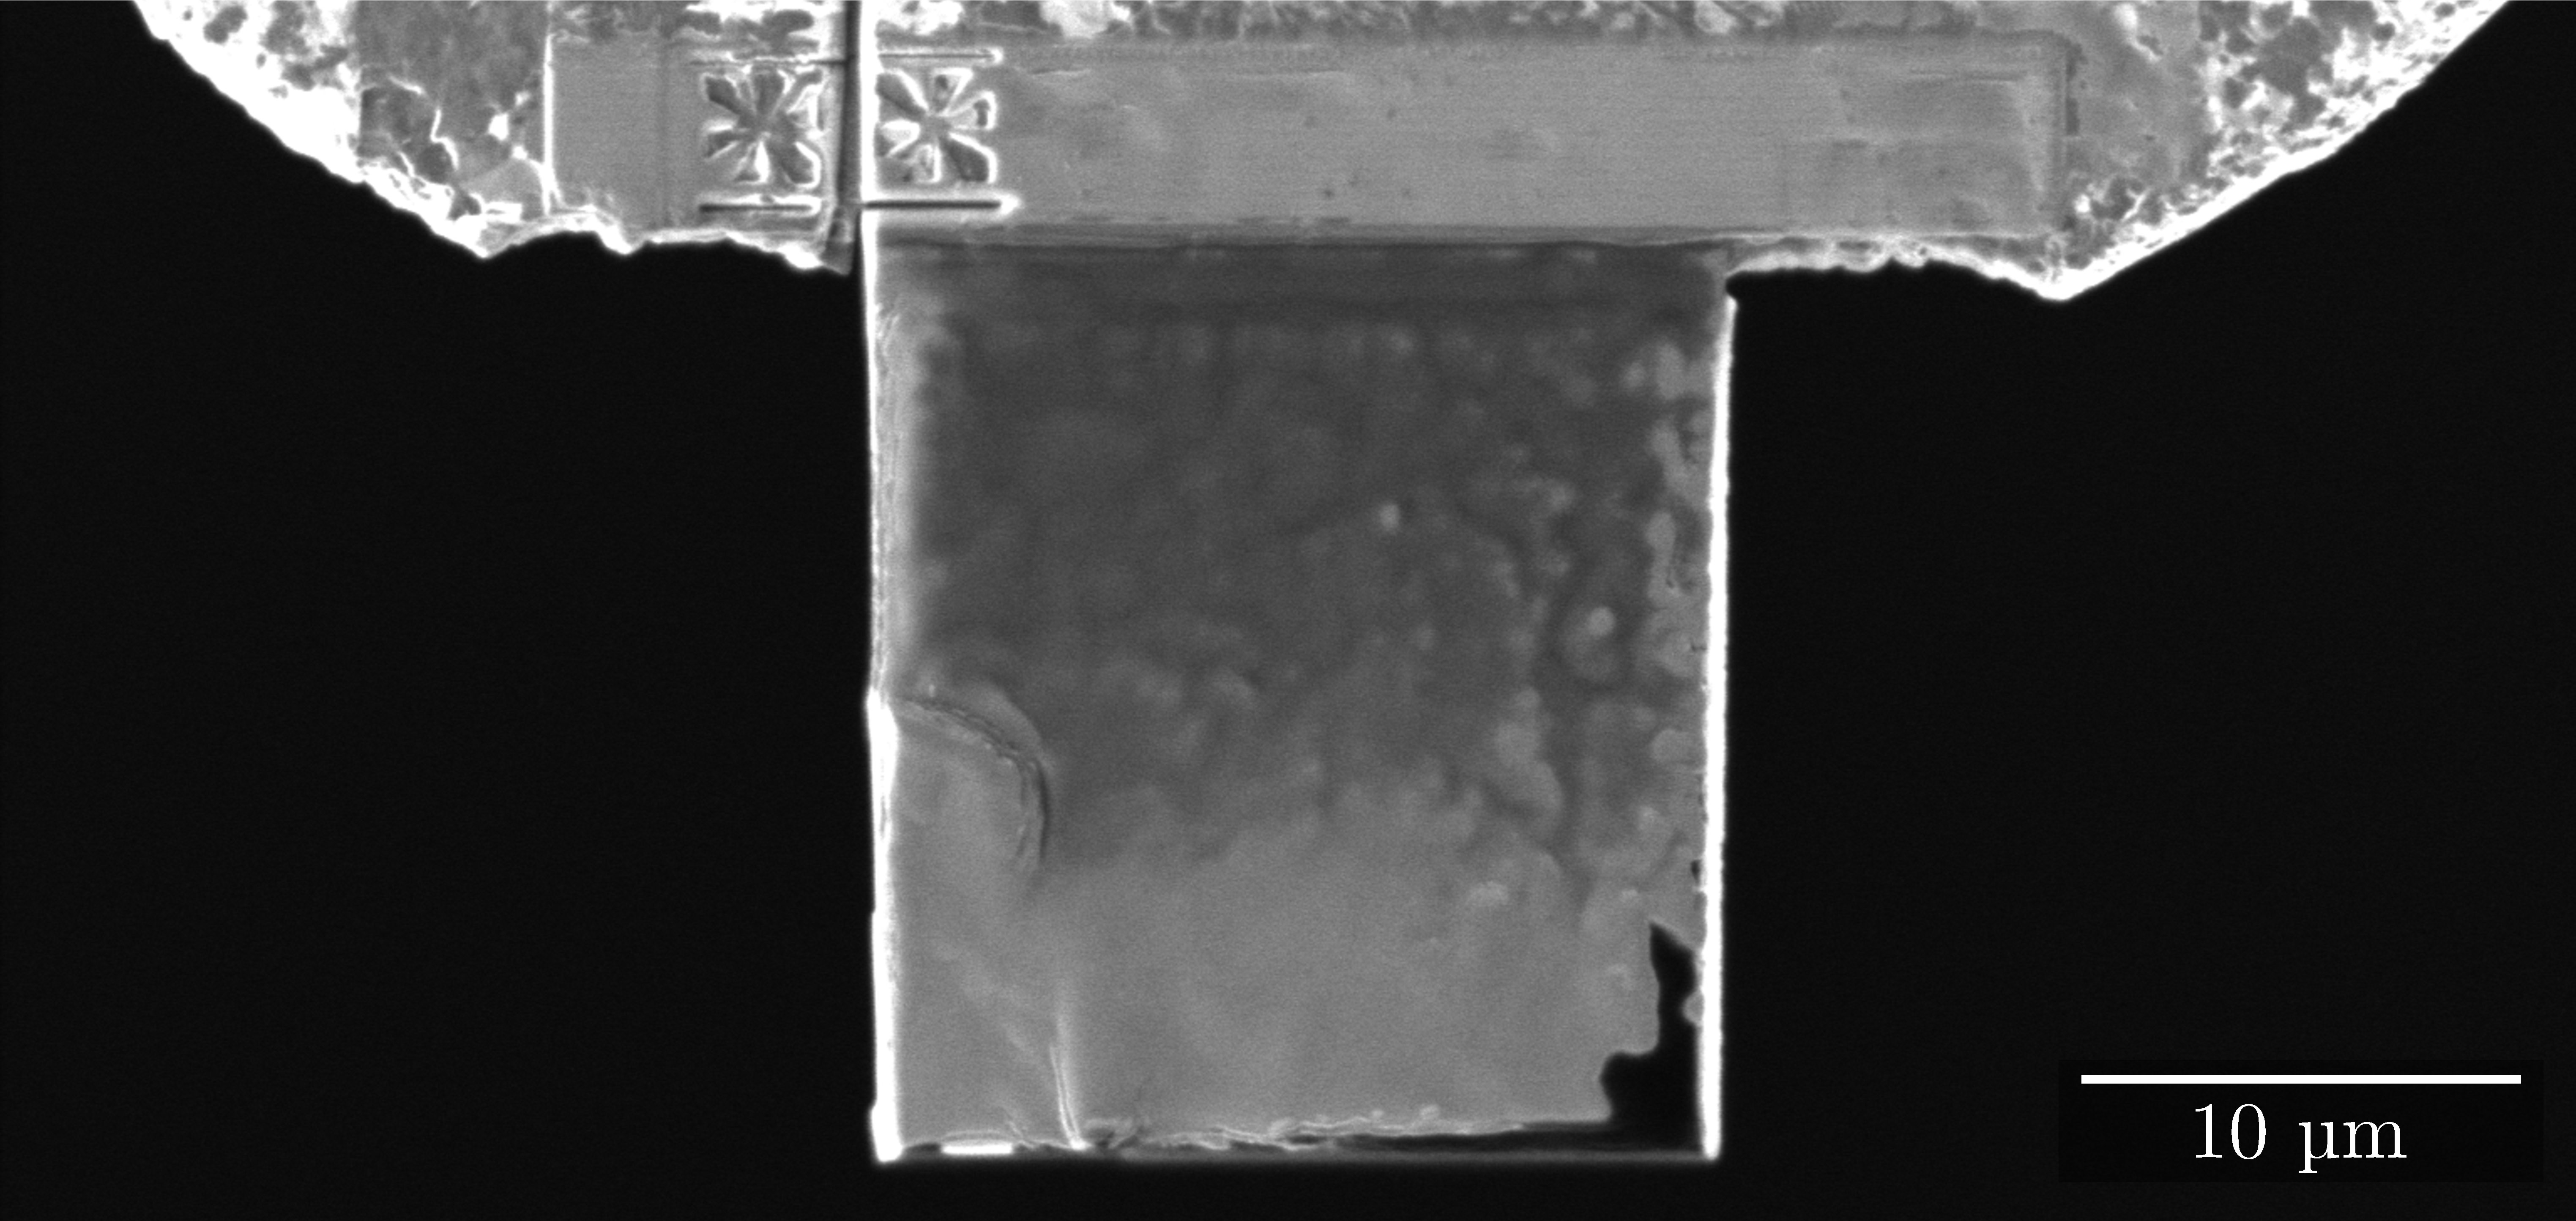
\includegraphics[width=0.65\linewidth]{methods/fib_liftout/ion_image.pdf}\hfill
      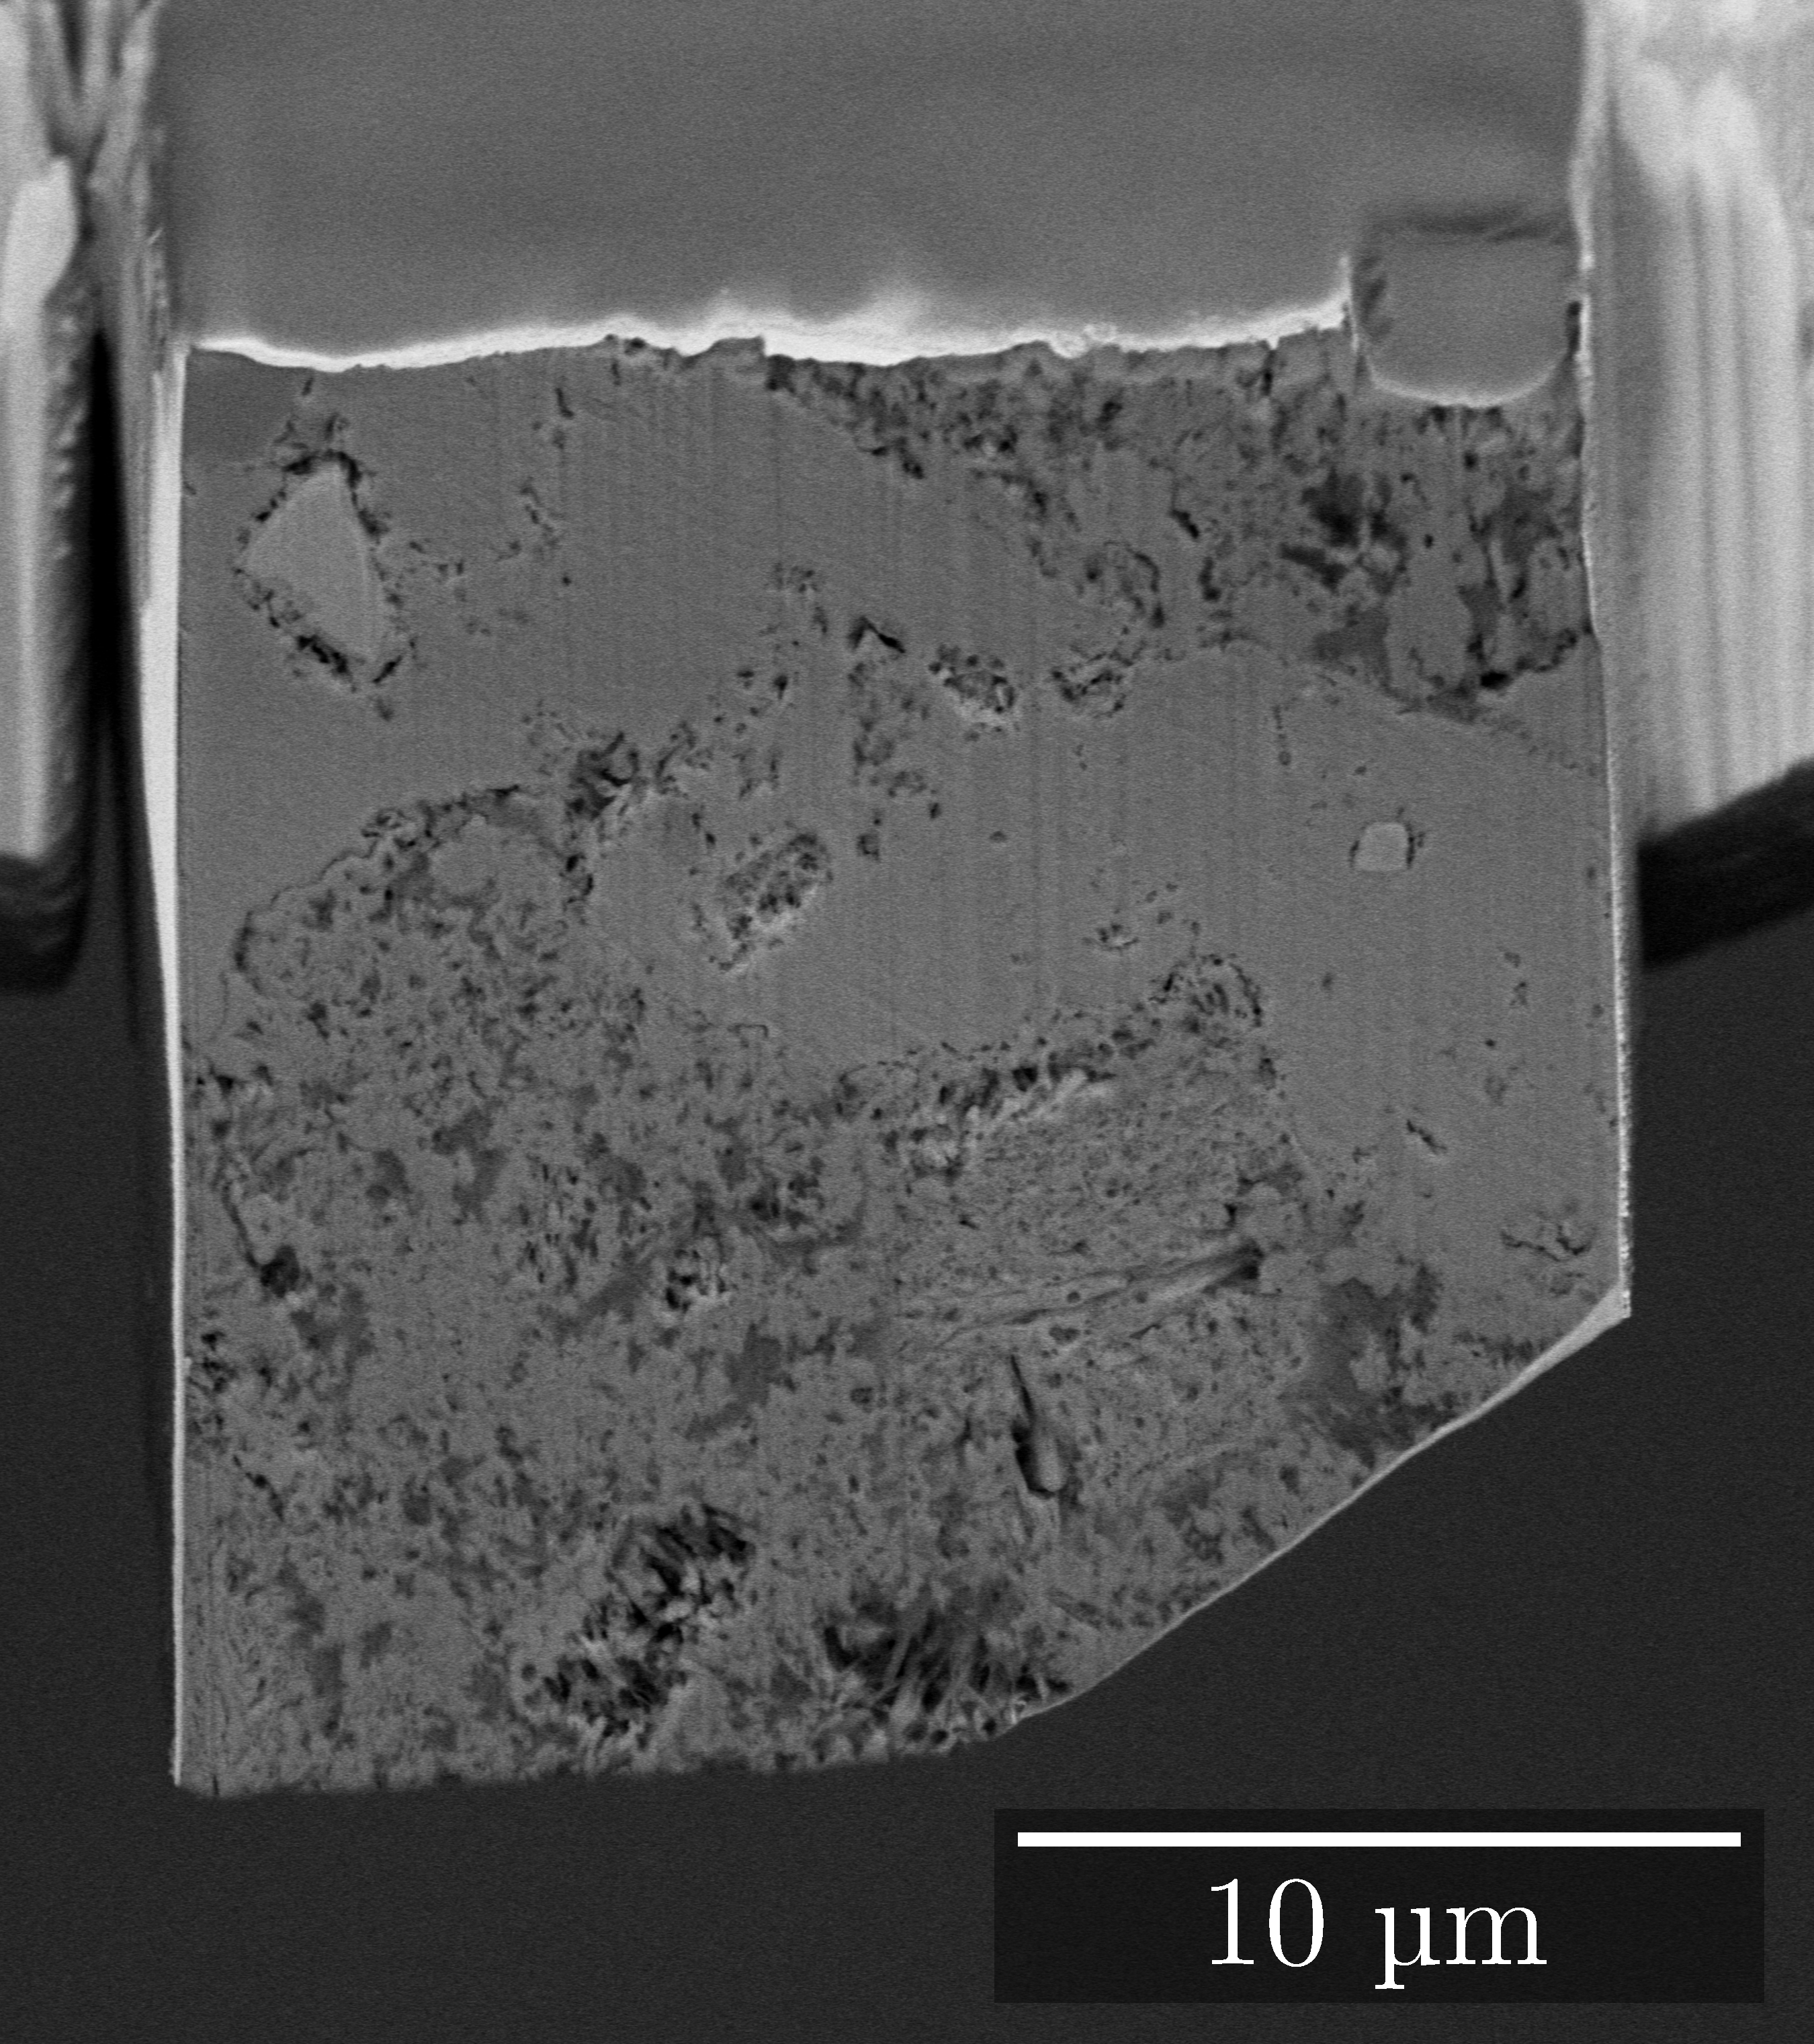
\includegraphics[width=0.27\linewidth]{methods/fib_liftout/bse_image.pdf}\\
      \footnotesize Top view (ion image, left) and\\front view (BSE, right)\\
    \end{column}
  \end{columns}
   \vfill
   \raggedleft\tiny\itshape F. Kleiner, C. Rößler, H.-M. Ludwig, `A FIB-SEM Protocol for High-Resolution Imaging Combined with EDX Analysis of Cement-Based Materials with Minimized Damage', 2025, \doi{10.71758/refodat.52}
\end{frame}

\subsection{fs-Laser Preparation}
\begin{frame}{3D Nano Tomography (FIB-nT) - fs-Laser Preparation}
  \begin{columns}
    \begin{column}{0.5\textwidth}
      \textbf{Challenges:}
      \begin{itemize}
        \item Lift-out technique results in very small volumes\\($20\,\times\,20\,\times\,20\,$µm³).
      \end{itemize}
      \textbf{The Solution:}
      \begin{itemize}
        \item Pre-preparation with fs-laser enables the preparation of large trenches ($0.6\,\times\,1.0\,$mm²).
      \end{itemize}
    \end{column}
    \begin{column}{0.5\textwidth}
      \centering
      \animategraphics[palindrome,poster=6,autoplay,width=0.49\linewidth]{5}{methods/laser_prep/tilt}{0}{6}\hfill
      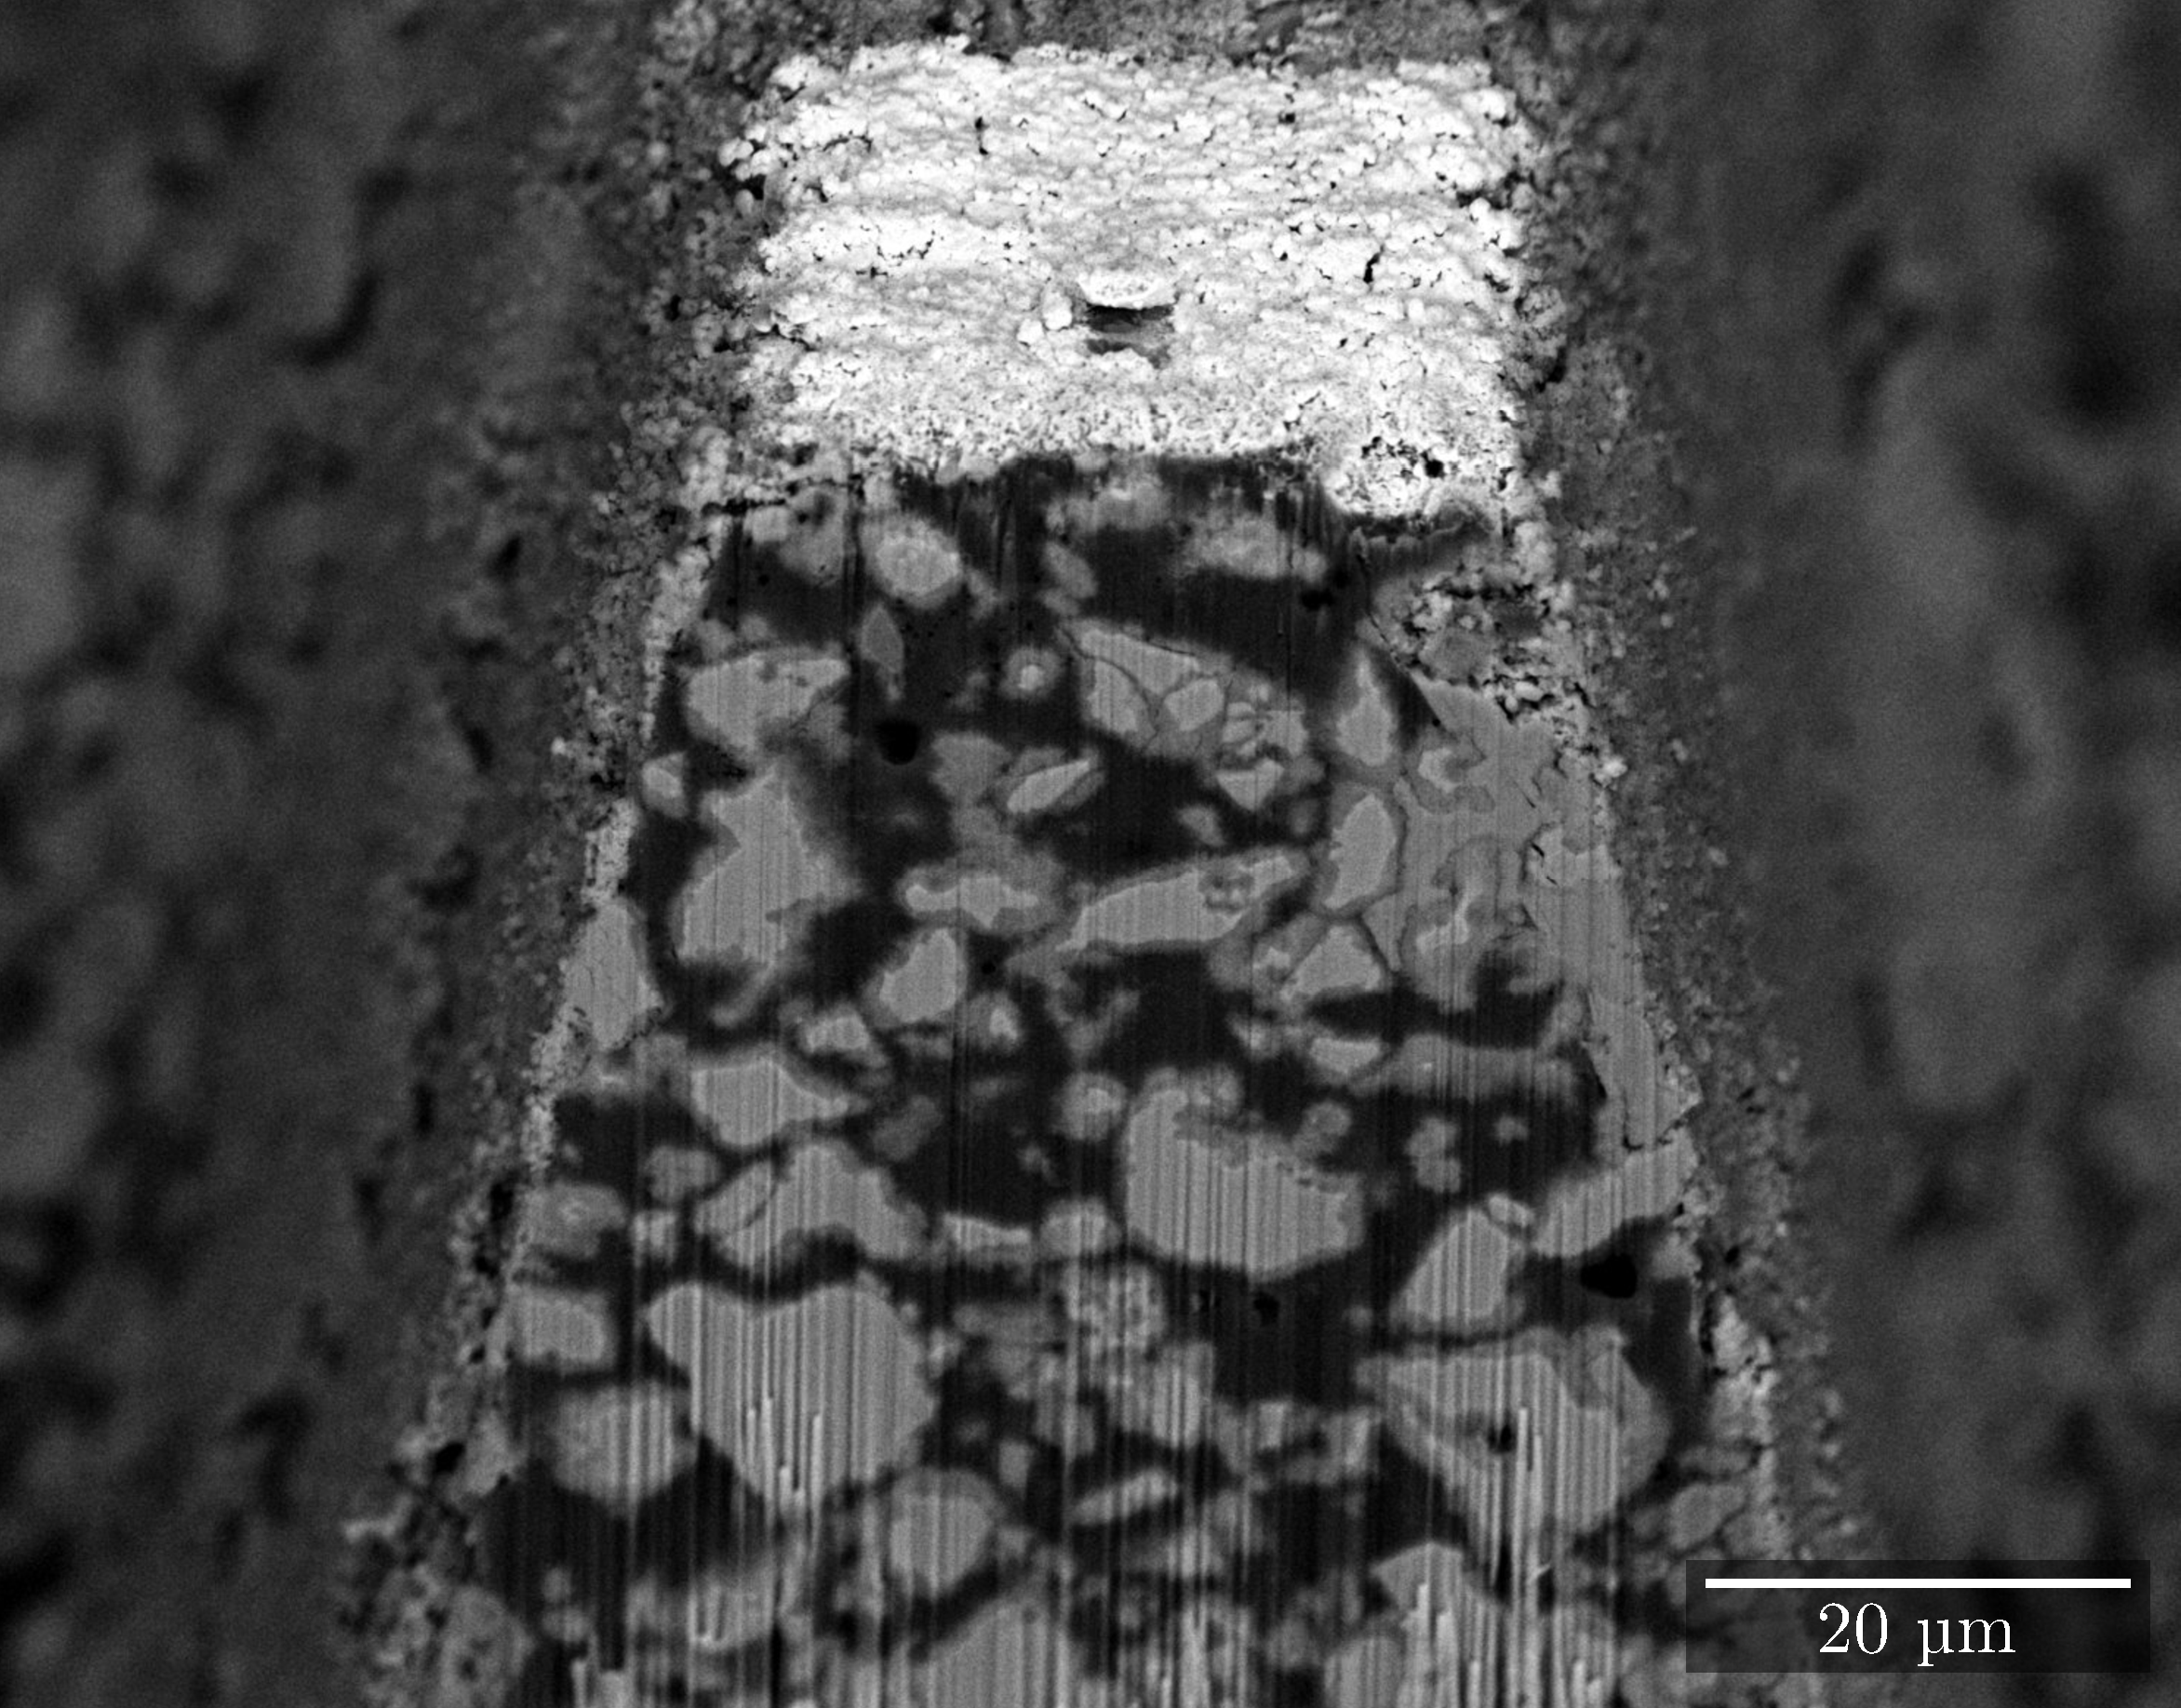
\includegraphics[width=0.49\linewidth]{methods/laser_prep/C3S_7d_Laser_prep_069.pdf}\\
      \footnotesize Laser trenches (left) and\\fresh FIB slice (right)\\
    \end{column}
  \end{columns}
  \vfill\raggedleft\tiny\itshape unpublished
\end{frame}

\section{Pore Space Analysis}
\subsection{LT-DSC vs. MIP}
\begin{frame}{Pore Space Analysis (LT-DSC vs. MIP)}
  \begin{columns}
    \begin{column}{0.5\textwidth}
      \textbf{LT-DSC Evaluation:}
      \begin{itemize}
        \item Determination of pore volume via the enthalpy of fusion ($\Delta H_{\mathrm{fus}}$).
        \item Differentiation between gel and capillary pores is possible.
        \item Linear decrease in capillary porosity with a simultaneous increase in gel porosity.
      \end{itemize}
      \textbf{MIP:}
      \begin{itemize}
        \item Primarily captures capillary pores ($>10$\,nm).
        \item Ink-bottle effects.
      \end{itemize}
    \end{column}
    \begin{column}{0.5\textwidth}
      \centering
      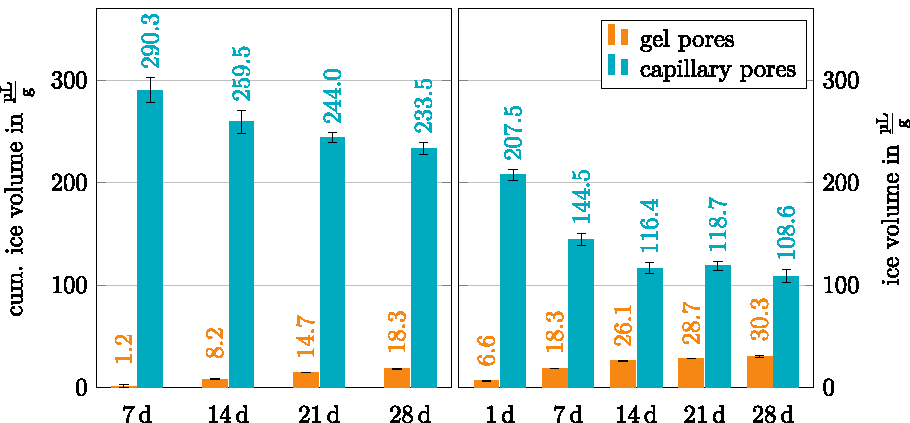
\includegraphics[width=\linewidth]{./graphics/pores/pores.pdf}\\
      \footnotesize Correlation between gel and capillary pore volume\\during progressive hydration.\\
    \end{column}
  \end{columns}
  \vfill\raggedleft\tiny\itshape unpublished
\end{frame}

\subsection{3D Nano-Pore Analysis (FIB-nT)}
\begin{frame}{3D Nano-Pore Analysis (FIB-nT)}
  \begin{columns}
    \begin{column}{0.5\textwidth}
      \begin{itemize}
        \item Direct visualisation of porosity within the dense C-S-H.
        \item 3D reconstruction from a high-resolution FIB-nT dataset.
        \item Dominant pore radius at $\approx 10.8$\,nm.
        \item Good agreement with LT-DSC/MIP and ArBIB sections.
      \end{itemize}
    \end{column}
    \begin{column}{0.5\textwidth}
      \centering
      \animategraphics[palindrome,autoplay,width=0.9\linewidth]{10}{fibnt-datasets/vol_ani/volume_}{00}{14}\\
      \footnotesize 3D reconstruction of the pore space (grey)\\in C-S-H (red).
    \end{column}
  \end{columns}
  \vfill\raggedleft\tiny\itshape unpublished
\end{frame}

\section{Summary}
\begin{frame}{Summary}
  \textbf{This thesis provides examples for the application of:}
  \begin{itemize}
    \item Correlative microscopy for cement-based materials.
    \begin{itemize}
        \item The combination (LA-ICP-MS + EDX, HLT + EBSD, NI + EDX) provides insights that individual methods cannot achieve.
    \end{itemize}
    \item Optimised preparation (ArBIB) and 3D analytical methods (FIB-nT).
    \item Automated quantitative image analysis methods for hydrate layer and particle distance measurements.
    \item Pore structure analysis of nanoporosity using FIB-nT and LT-DSC.
  \end{itemize}
\end{frame} 

\appendix

\begin{frame}{Acronyms}
  \begin{multicols}{2}
    \scriptsize
    \begin{description}[LA-ICP-MS]
      \item[ArBIB] Argon Broad Ion Beam
      \item[BSE] Backscattered Electron
      \item[C-A-S-H] Calcium Aluminate Silicate Hydrate
      \item[CEM~I] Portland cement as defined in DIN EN 197-1
      \item[C-S-H] Calcium Silicate Hydrate
      \item[\ce{C2S}] Dicalcium Silicate
      \item[\ce{C3S}] Tricalcium Silicate
      \item[EBSD] Electron Backscatter Diffraction
      \item[EDX] Energy-Dispersive X-ray Spectroscopy
      \item[FIB] Focussed Ion Beam
      \item[FIB-nT] FIB nano Tomography
      \item[fs-Laser] Femtosecond Laser
      \item[HLT] Hydrate Layer Thickness
      \item[IPF] Inverse Pole Figure
      \item[ITZ] Interfacial Transition Zone
      \item[LA-ICP-MS] Laser Ablation - Inductively Coupled Plasma - Mass Spectrometry
      \item[LC$^3$] Limestone Calcined Clay Cement
      \item[LT-DSC] Low Temperature - Differential Scanning Calorimetry
      \item[MIP] Mercury Intrusion Porosimetry
      \item[NI] Nanoindentation
      \item[PCE] Polycarboxylate Ether
      \item[PUS] Power Ultrasound
      \item[SE] Secondary Electron
      \item[SEM] Scanning Electron Microscope
      \item[SLIC] Simple Linear Iterative Clustering
      \item[UMAP] Uniform Manifold Approximation
    \end{description}
  \end{multicols}
\end{frame}

\end{document}